\section{Julius}\label{Julius}
次にJuliusを紹介します。コマンド1つで試せるようにしてあります。下のようにターミナルにコマンドを打ちましょう。\\
\code{run-linux-gmm.sh}\\
このコマンドを打つと、いくらかシステム情報が表示された後、「<<please speak>>」という文字列が現れます( 図\ref{juliusの使い方})。

\begin{figure}[H]
\begin{center}
    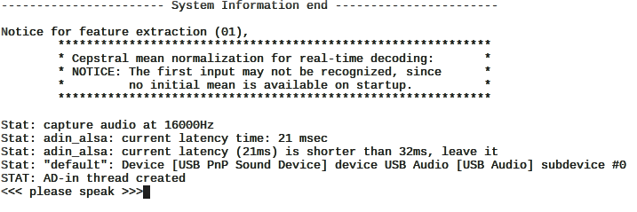
\includegraphics[width=\linewidth]{images/chap06/text06-img009.png}
    \caption{juliusの使い方}
    \label{juliusの使い方}
\end{center}
\end{figure}

その後マイクに向かって話しかければ、話しかけた単語が文字列になって画面に表示されます。今回は試しに果物の名前を話しかけてみましょう。
\begin{center}
	りんご みかん ぶどう もも あけび あんず いちご いちじく かき スイカ\\すもも 	なし メロン
\end{center}
	
終了するときはCtrl+c(コントロールキーを押しながらcを押す)を使います。<<please speak>>と表示されなくなり、pi@raspberrypi:と表示されればOKです。

Juliusはうまく言葉を認識してくれましたか?おそらく、何度か間違えて認識したと思います。日本語には数多の単語がありますし、似た発音の単語もあるので、それらを完璧に認識することは難しいのです。これを解決するために、「単語辞書」を登録してみましょう。\\

\begin{tcolorbox}[title=\useOmetoi]
\begin{enumerate}
\item ターミナルにrun-linux-gmm.shと入力し、Juliusを試してみましょう。\\<<please speak>>と表示されたらマイクに向かって果物の名前を5つ話しかけましょう。\\何個認識されましたか?\\ \underline{答え.\hspace{0.8\linewidth}}
\end{enumerate}
\end{tcolorbox}